\section{Úvod}
\label{sec:Úvod}

Matematické kyvadlo je nejjednodušším typem kyvadla. Máme hmotný bod o hmotnosti $m$ zavěšený na provázku délky $l$ zanedbatelné hmotnosti. Tření a odpor vzduchu nezapočítáváme. Tíhové pole považujeme za homogenní s tíhovým zrychlením $g$.

\subsection*{Pohybová rovnice}
\label{sec:Pohybová rovnice}
Hmotný bod se pohybuje po kružnici o poloměru $l$ a jeho pohyb popisujeme aktuálním úhlem $\varphi(t)$, který měří výchylku z dolní rovnovážné polohy. Pro zrychlení platí $a=l\varepsilon=l\dot{\omega}=l\ddot{\varphi}$ a pro vratnou sílu platí $F=-mg\sin\varphi$. Použijeme 2. Newtonův zákon: $F=ma$.
\begin{equation*}
ma=ml\ddot{\varphi}=F=-mg\sin\varphi\\
\end{equation*}
Můžeme pokrátit $m$ z naší rovnice a vydělíme celou rovnici $l$. Pak vše převedeme na jednu stranu. Dostáváme pohybovou rovnici matematického kyvadla.
\begin{equation}
\label{pohyb}
\boxed{\ddot{\varphi}+\frac{g}{l}\sin\varphi=0}
\end{equation}
Vidíme, že naše rovnice je nelineární diferenciální rovnice druhého řádu. Pokud budeme brát v úvahu jen malé výchylky z rovnovážné polohy, můžeme rovnici linearizovat.
\begin{equation}
\label{linrce}
\ddot{\varphi}+\frac{g}{l}\varphi=0
\end{equation}
Využili jsme Taylorova rozvoje $\sin\varphi$:
\begin{equation*}
\sin\varphi = \varphi-\frac{\varphi^3}{6}+\frac{\varphi^5}{120}+O\left(\varphi^6\right).
\end{equation*}
Kde jsme vzali jen první člen, neboť nás zajímají jen malé výchylky. Když vezmeme počáteční podmínku $\varphi(t_0=0)=\varphi_0$, tak řešení rovnice ($\ref{linrce}$) vypadá takto
\begin{equation}
\label{reslinrce}
\varphi=\varphi_0\cos\sqrt{\frac{g}{l}}t.
\end{equation}
Jak můžeme vidět, rovnice ($\ref{reslinrce}$) odpovídá rovnici harmonického oscilátoru s amplitudou $\varphi_0$ a s úhlovou frekvencí malých harmonických kmitů $\omega = \sqrt{\frac{g}{l}}$.
Periodě matematického kyvadla při malých výchylkách pak odpovídá
\begin{equation}
\label{malperiod}
T=2\pi\sqrt{\frac{l}{g}}.
\end{equation}

\section{Perioda oscilací}
\label{sec:Perioda oscilací}

\subsection{Eliptický integrál}
\label{sec:Eliptický integrál}
Eliptický integrál nám poskytuje exaktní řešení nelinearizované rovnice ($\ref{pohyb}$). Když rovnici ($\ref{pohyb}$) vynásobíme $\frac{d\varphi}{dt}$, tak získáme:
\begin{equation*}
\frac{d\varphi}{dt}\left(\ddot{\varphi}+\frac{g}{l}\sin\varphi\right)=\frac{d}{dt}\left(\frac{1}{2}\dot{\varphi}^2-\frac{g}{l}\cos\varphi\right)=0.
\end{equation*}
Po integraci dostáváme první integrál pohybu pohybové rovnice ($\ref{pohyb}$).
\begin{equation}
\frac{1}{2}\dot{\varphi}^2-\frac{g}{l}\cos\varphi=C
\end{equation}
Protože chceme, aby kyvadlo mělo na počátku nulovou rychlost ($\dot{\varphi}=0$, pro $\varphi=\varphi_0$, kde $\varphi_0$ je počáteční úhel), můžeme dopočítat konstantu $C$, což nám dává $C=-\frac{g}{l}\cos\varphi_0$. Dosadíme konstantu $C$ a upravíme.
\begin{equation}
\label{intpohyb}
\dot{\varphi}=\frac{d\varphi}{dt}=\sqrt{\frac{2g}{l}}\sqrt{\cos\varphi-\cos\varphi_0}
\end{equation}
Využijeme větu o derivaci inverzní funkce na ($\ref{intpohyb}$) a vynásobíme ji $d\varphi$.
\begin{equation}
dt=\frac{d\varphi}{\sqrt{\frac{2g}{l}}\sqrt{\cos\varphi-\cos\varphi_0}}
\end{equation}
Budeme integrovat od $\varphi=0$ do $\varphi=\varphi_0$. Tento interval odpovídá čtvrtině periody.
\begin{equation}
\frac{T}{4}=\int_{0}^{\varphi_0}\frac{\,d\varphi}{\sqrt{\frac{2g}{l}}\sqrt{\cos\varphi-\cos\varphi_0}}
\end{equation}
Pomocí substituce $\cos\varphi=1-2\sin^2\theta$ ($\theta=\frac{\varphi}{2}$) a dalších úprav, se nám podaří získat eliptický integrál, díky němuž jsme schopni vypočítat periodu $T$ matematického kyvadla.
\begin{equation}
\label{integ}
T=4\sqrt{\frac{l}{g}}\int_{0}^{\frac{\pi}{2}}\frac{\,d\theta}{\sqrt{1-k^2\sin^2\theta}},
\end{equation}
kde $k=\sin\frac{\varphi_0}{2}$.
Uděláme Taylorův rozvoj $\frac{1}{\sqrt{1-k^2\sin^2\theta}}$, čímž si usnadňujeme práci s integrálem, ale musíme počítat s tím, že budeme získávat jeho aproximovanou hodnotu.
\begin{equation}
\label{rozvoj}
\frac{1}{\sqrt{1-k^2\sin^2\theta}}\approx1+\frac{1}{8} \varphi_0 ^2 \sin ^2\theta+\frac{1}{384} \varphi_0 ^4 \left(9 \sin ^4\theta-4 \sin
   ^2\theta \right)
\end{equation}
Teď už jen ($\ref{rozvoj}$) vložíme do ($\ref{integ}$) a dostaneme:
\begin{equation}
T=4\sqrt{\frac{l}{g}}\int_{0}^{\frac{\pi}{2}}\frac{\,d\theta}{\sqrt{1-k^2\sin^2\theta}}\approx2\pi\sqrt{\frac{l}{g}}\left(1+\frac{1}{16}\varphi_0^2+\frac{11}{3072}\varphi_0^4\right).
\end{equation}

\section{Numerické řešení}
\label{sec:Numerické řešení}

V předchozích kapitolách jsme dospěli k rovnici $\eqref{pohyb}$. Vzhledem k jednotě značení v této sekci ji přepišme jako:
\begin{equation}
\label{rovnice}
\boxed{\frac{\diff^{2} y}{\diff t ^{2}} + \frac{g}{l}\sin y=0},
\end{equation}
kde $y(t)$ je výchylka (orientovaný úhel) kyvadla v čase $t$.
Pokusme se nyní tuto rovnici řešit pomocí numerických metod. K tomu využijeme prostředí \textit{Mathematica}.\footnote{všechny přiložené kódy jsou napsané v Mathematica 12.02}
Pro jednoduchost předpokládejme délku kyvadla $l=1$ \si{m}, hmotnost $m = 1$ \si{kg}, tíhové zrychlení jako $g = 9.81$ \si{m.s^{-2}}, počáteční výchylku $y(0)=y_{0}=1$ \si{rad} a čas $1$ \si{s} $\leq t \leq$ 10 \si{s}, po který budeme sledovat pohyb matematického kyvadla.
\begin{lstlisting}[language=Mathematica, caption=Konstanty]
g = 9.81;
l = 1;
poc = 1;
time = {t, 0, 10};
\end{lstlisting}

\subsection{Zachování energie}
\label{sec:Zachování energie}
Hmotný bod na závěsu vychýlíme z rovnovážné polohy o úhel $y_{0}=1$ \si{rad} a pustíme bez udělení počáteční rychlosti $y'(0)=0$. Dále zanedbávejme odpor prostředí apod. Kyvadlo se začne periodicky pohybovat s periodou $T$. Náš systém zachovává mechanickou energii:
\begin{equation}
E = \frac{1}{2} m [y'(t)]^{2}- \frac{g}{l} m \cos(y(t)),
\end{equation} 
která na počátku pohybu byla rovna:
\begin{equation}
E = E_{0} = - \frac{g}{l} m \cos(y_{0}).
\end{equation} 
Tedy v průběhu numerického řešení bychom očekávali splnění rovnice:
\begin{equation}
\label{ener}
\boxed{- \frac{g}{l}  \cos(y_{0}) = \frac{1}{2} [y'(t)]^{2} - \frac{g}{l} \cos(y(t))}
\end{equation} 
a to v každém čase $t$. Při hodnocení numerických metod je pro nás výhodné znázornit trajektorii $(y(t),y'(t))$\footnote{respektive trajektori $(q(t),p(t))$, kde $q$ je zobecněná souřadnice a $p$ je kanonická hybnost, ale v našem případě $q(t)=y(t)$ a $p(t)=y'(t)$, při uvážení $m=1$} řešení ve fázovém prostoru. Pokud fázovým portrétem bude uzavřená křivka, naše numerické řešení zachovává celkovou energii systému.

\subsection{Metody}
\label{sec:Metody}

Na příkladech numerických řešení rovnice $\eqref{rovnice}$ si ukážeme úskalí používání numerických metod při konfrontaci se zachováním periodicity a při zachování energie apod. 

\begin{description}
\item[Automatická metoda zvolená softwarem] Podívejme se na řešení s automatickým výběrem metody v příkazu \texttt{NDSolve}:

\begin{lstlisting}[language=Mathematica]
NDSolve[{y''[t]  + g/l*Sin[y[t]] == 0, y[0] == poc,y'[0] == 0}, y, time];
\end{lstlisting}

Na obrázku $\eqref{fig:ND1}$ vidíme periodicitu řešení. Z $\eqref{fig:ND2}$ a $\eqref{fig:ND3}$ plyne, že řešení poměrně zachovává energii s přesností $10^{-5}$.

\begin{figure}[h]
  \centering
  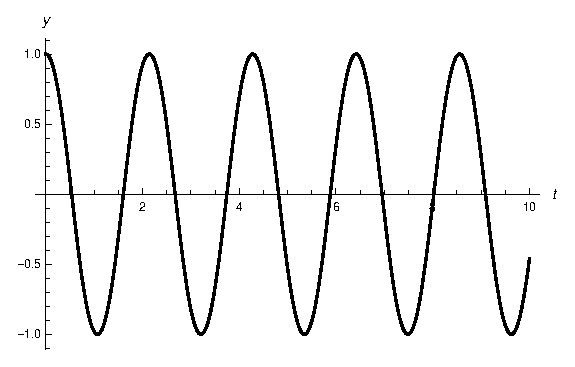
\includegraphics[width=10cm]{figures/ND1.eps}
  \caption{Časová závislost výchylky na čase}
  \label{fig:ND1}
\end{figure}

\begin{figure}[h]
  \centering
  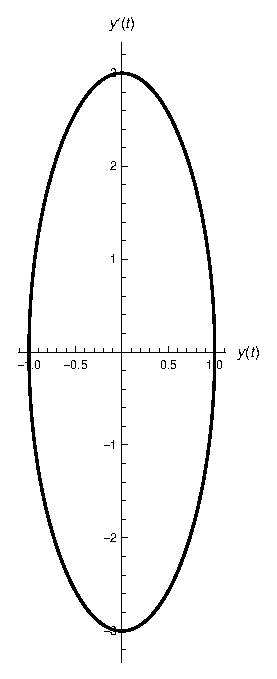
\includegraphics[width=3cm]{figures/ND2.eps}
  \caption{Fázový prostor}
  \label{fig:ND2}
\end{figure}

\begin{figure}[h]
  \centering
  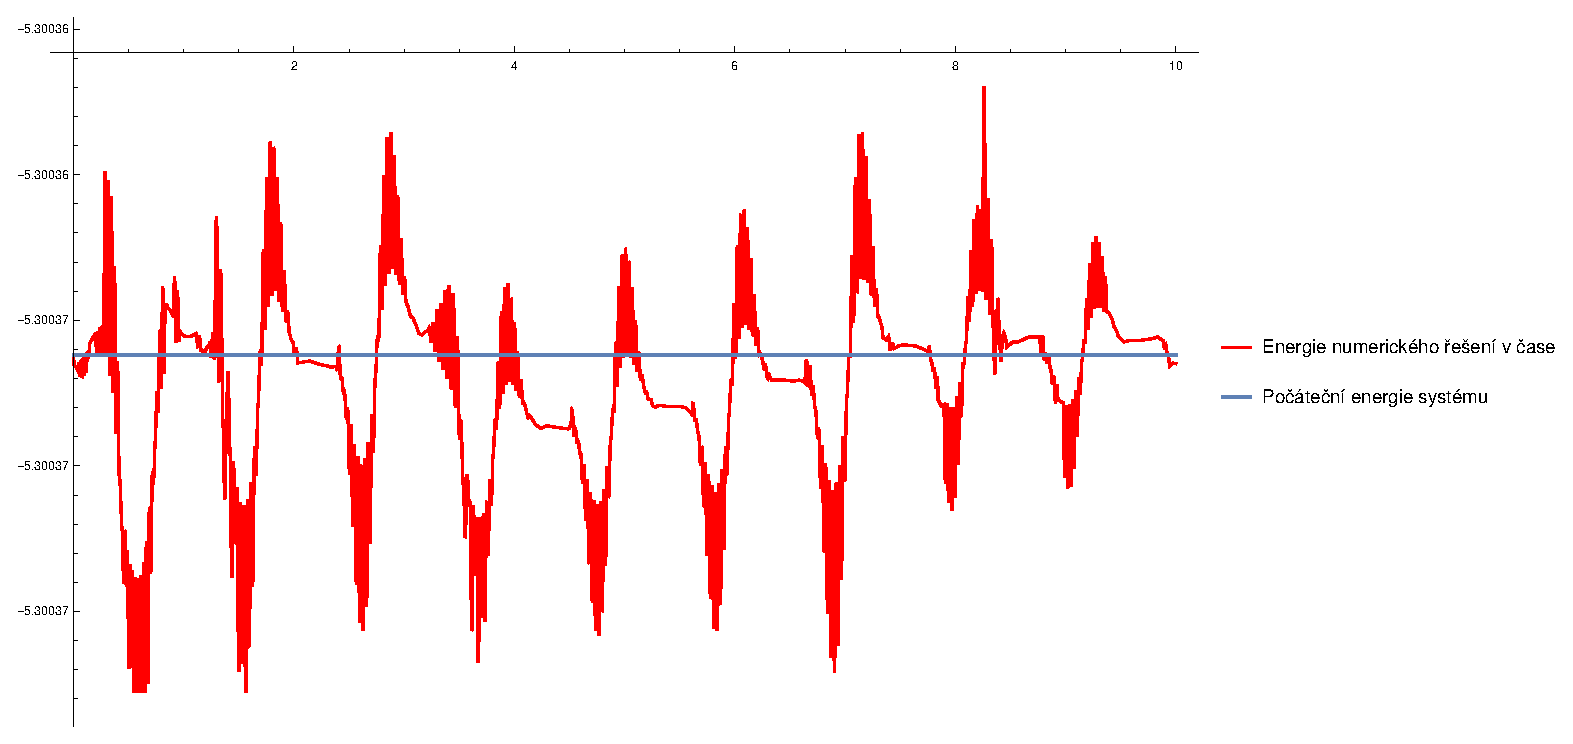
\includegraphics[width=15cm]{figures/ND3.eps}
  \caption{Zachování energie - rovnice $\eqref{ener}$}
  \label{fig:ND3}
\end{figure}

\item[Explicitní Eulerova metoda] 

Tato metoda je nejjednodušší a zároveň, jak si ukážeme, nejméně vhodná pro numerické řešení rovnice $\eqref{rovnice}$. Proto si ji pro ilustraci rozeberme trochu podrobněji. Mějme rovnoměrné (ekvidistantní) dělení $\left\lbrace t_{n} \right\rbrace $ intervalu $(0,10)$:
\begin{equation*}
t_{n} = n h , n \in \mathbb{N_{0}},
\end{equation*}
kde $h$ je velikost kroku. Dále aproximujme $y(t_{n}) \approx y_{n}$. Pak explicitní Eulerova metoda (jednokroková) pro rovnici\footnote{předpokládáme existenci řešení} $y'(t)=f(t,y(t))$ se dá vyjádřit jako\footnote{v našem případě ODR 2. řádu bychom převedli na soustavu ODR 1. řádu}:
\begin{equation*}
y_{n+1} = y_{n} + h f(t_{n},y_{n}).
\end{equation*}
Pro demonstraci získání "špatného" výsledku použijme:
\begin{lstlisting}[language=Mathematica,caption=Eulerova metoda]
NDSolve[{y''[t]+g/l*Sin[y[t]] == 0,y[0] == poc,y'[0] == 0},y, time, Method -> "ExplicitEuler", StartingStepSize -> 0.1,MaxStepSize -> 0.1, MaxSteps -> 100]
\end{lstlisting}

Výsledné numerické řešení naprosto ztrácí periodicitu - obrázek $\eqref{fig:EU1}$ a nezachovává energii $\eqref{fig:EU2}$, $\eqref{fig:EU3}$ - systém energii v čase získává.


\begin{figure}[h]
  \centering
  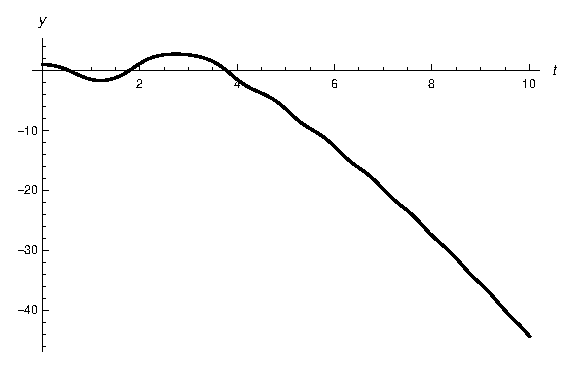
\includegraphics[width=10cm]{figures/EU1.eps}
  \caption{Eulerova metoda - časová závislost výchylky na čase}
  \label{fig:EU1}
\end{figure}

\begin{figure}[h]
  \centering
  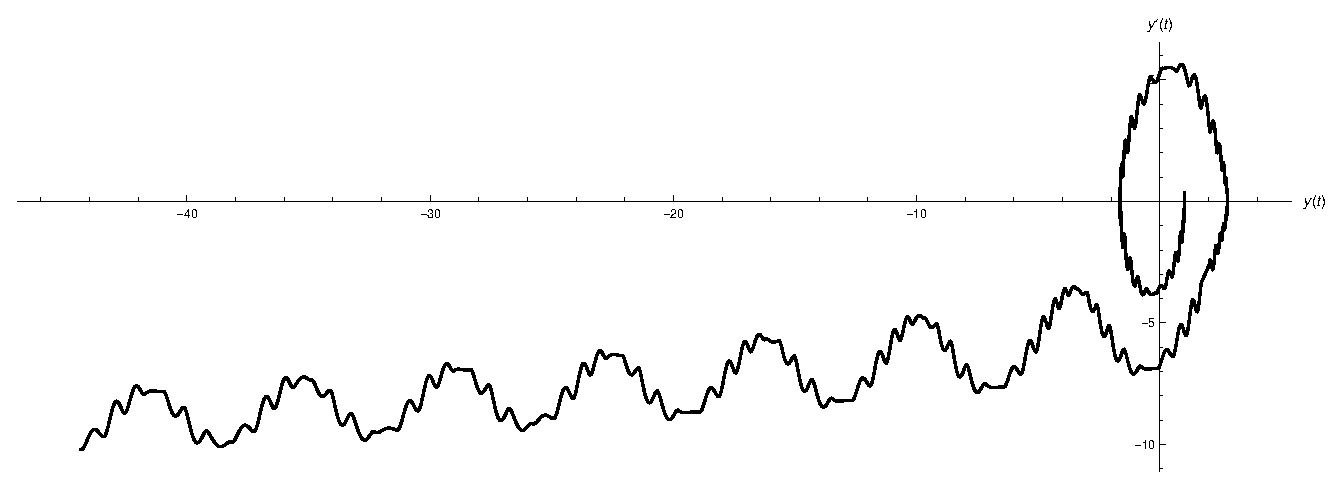
\includegraphics[width=15cm]{figures/EU2.eps}
  \caption{Eulerova metoda - fázový prostor}
  \label{fig:EU2}
\end{figure}

\begin{figure}[h]
  \centering
  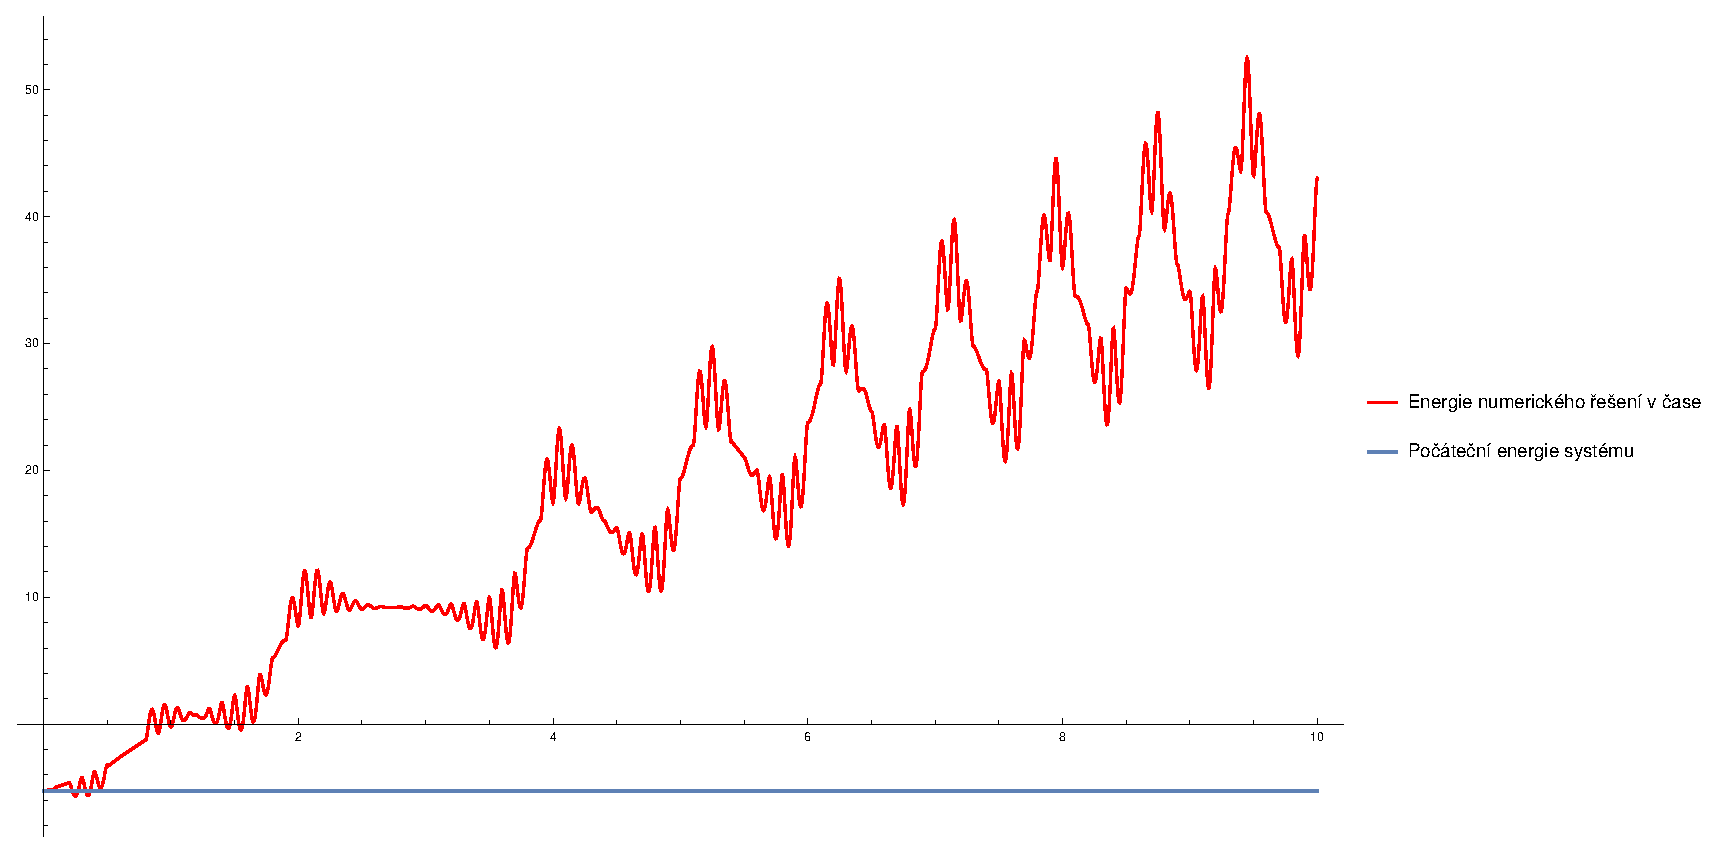
\includegraphics[width=15cm]{figures/EU3.eps}
  \caption{Eulerova metoda - energie}
  \label{fig:EU3}
\end{figure}

\item[Metody snažící se zachovat celkovou energii] 
Nyní použijeme sofistikovanější metody založené na Runge-Kuttových metodách. Pro ilustraci napišme explicitní Runge-Kuttovu metodu 4. řádu (zachováme značení jako výše) pro rovnici~$y'(t)=f(t,y(t))$:
\begin{align*}
K_{1} & = f(t_{n},y_{n}), \\
K_{2} & = f \left(  t_{n}+\frac{h}{2},y_{n}+h\frac{K_{1}}{2} \right),  \\
K_{3} & = f \left(  t_{n}+\frac{h}{2},y_{n}+h\frac{K_{2}}{2} \right), \\
K_{4} & = f(t_{n}+h,y_{n}+h K_{3}), \\
y_{n+1} & = y_{n}+\frac{1}{6}(K_{1}+2K_{2}+2K_{3}+K_{4}).\\
\end{align*}

Konkrétně použijeme metodu \texttt{SymplecticPartitionedRungeKutta}, která ovšem vyžaduje přejít do Hamiltonova formalismu:
\begin{lstlisting}[language=Mathematica,caption=Hamiltonův formalismus]
H = p[t]^2/2 - g/l *Cos[q[t]];
eqs = {p'[t] == -D[H, q[t]], q'[t] == D[H, p[t]]};
ics = {p[0] == 0, q[0] == poc};
vars = {q[t], p[t]};
\end{lstlisting}
Máme časově nezávislý hamiltonián - zachovává se v čase (integrál pohybu):
\begin{equation}
H = \frac{p^{2}}{2m} -\frac{g}{l} m \cos(q).
\end{equation}
Implementace metody:
\begin{lstlisting}[language=Mathematica]
NDSolve[{eqs, ics}, vars, time,Method ->{"SymplecticPartitionedRungeKutta","DifferenceOrder" -> 4, "PositionVariables" -> {q[t]}}];
\end{lstlisting}

%\begin{figure}[h]
%  \centering
%  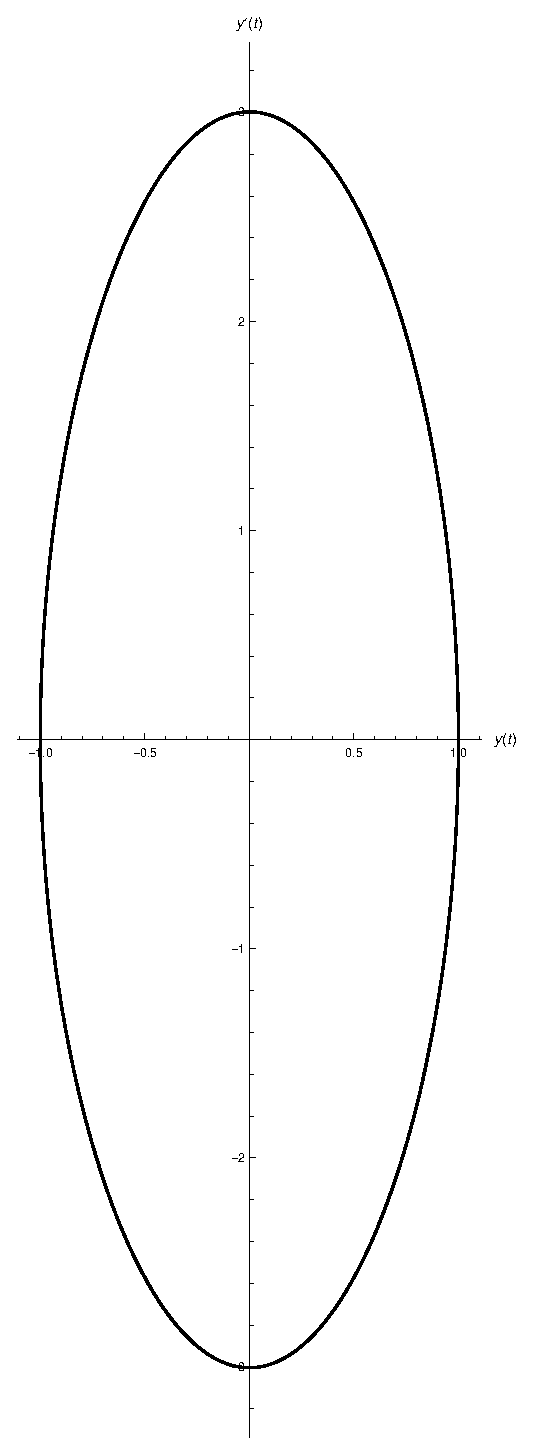
\includegraphics[width=12cm]{figures/SymRK2.eps}
%  \caption{fázový prostor}
%\end{figure}

Pro porovnání zkusme ještě jiný přístup pomocí \texttt{Projection}:
\begin{lstlisting}[language=Mathematica]
NDSolve[{y''[t] + g/l *Sin[y[t]] == 0, y[0] == poc,y'[0] == 0}, y, time,  Method -> {"Projection", Method -> "ExplicitRungeKutta", "Invariants" -> -g/l *Cos[poc]}];
\end{lstlisting}


V tabulce $\eqref{fig:tab}$ je porovnání všech použitých metod (vyjma Eulerovy metody). Nejlépe z použitých metod vychází \texttt{SymplecticRungeKutta}, která zachovává energii s přesností přibližně $10^{-6}$. Automaticky vybraná metoda při příkazu \texttt{NDSolve} zachovává energii asi s přesností $10^{-5}$. Posledně zmíněná metoda \texttt{Projection} zachovává energii s přesností okolo $10^{-3}$ tedy s menší přesností než první dvě metody.

\begin{figure}[h]
  \centering
  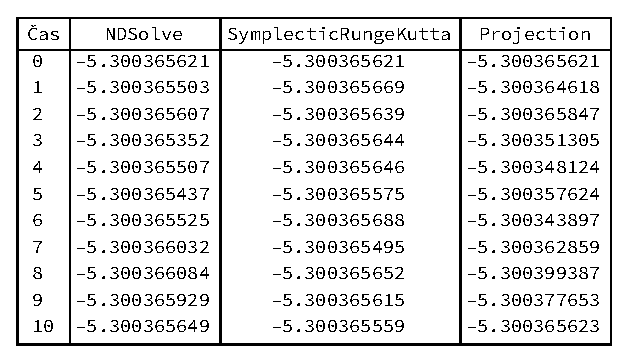
\includegraphics[width=10cm]{figures/TAB1.eps}
  \caption{Porovnání metod podle energií v čase}
  \label{fig:tab}
\end{figure}



\end{description}

\subsection{Perioda kyvadla}
\label{sec:Perioda}

Periodu matematického kyvadla $T$ určíme jako čtyřnásobek času, za který hmotný bod z počáteční výchylky proběhne rovnovážnou polohu. K jeho stanovení využijeme metod ukázaných výše, přímou integraci eliptického integrálu a aproximaci odvozenou v prvních kapitolách:
\begin{equation}
\label{aproxperiod}
T= 2 \pi \sqrt{\frac{l}{g}} \left( 1 + \frac{y_{0}^{2}}{16} + \frac{11y_{0}^{2}}{3072} \right) .
\end{equation}
Pro porovnání budeme periodu určovat při různých počátečních výchylkách $y_{0}$ a dodejme ještě velikost periody pro linearizovanou rovnici:
\begin{equation}
\label{aproxperiod}
T= 2 \pi \sqrt{\frac{l}{g}}.
\end{equation}

\begin{figure}[h]
  \centering
  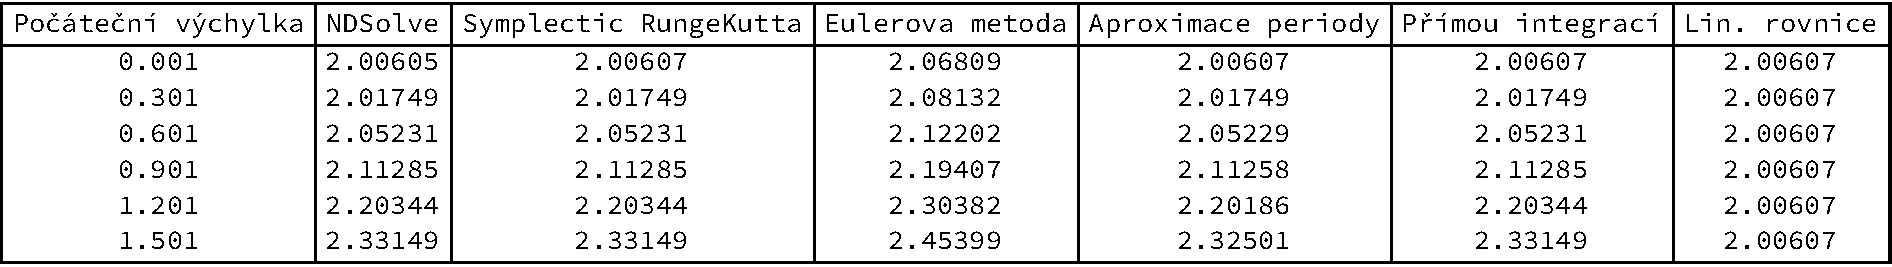
\includegraphics[width=17cm]{figures/perTab.pdf}
  \caption{Velikost periody $T$ pro různé metody v závislosti na počáteční výchylce $y_{0}$}
  \label{fig:pertab}
\end{figure}

\begin{figure}[h]
  \centering
  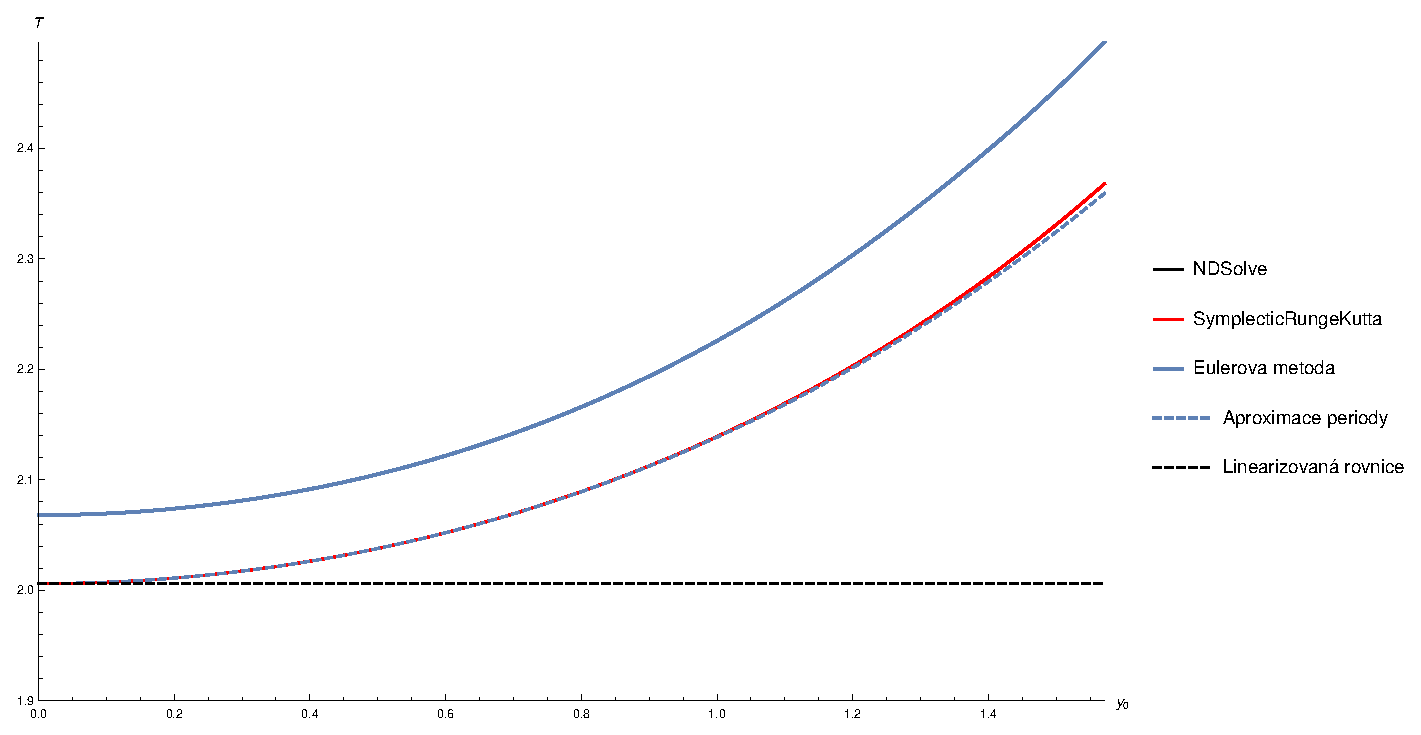
\includegraphics[width=17cm]{figures/PER2+LIN.eps}
  \caption{Velikost periody $T$ pro různé metody v závislosti na počáteční výchylce $y_{0}$}
  \label{fig:per}
\end{figure}

Z obrázku $\eqref{fig:per}$ a z tabulky $\eqref{fig:pertab}$ je patrné, že Eulerova metoda se výrazně odlišuje od zbylých. Metody \texttt{NDSolve} a \texttt{SymplecticPartitionedRungeKutta} jsou velmi přesné, překvapivě aproximace periody $\eqref{aproxperiod}$ je také poměrně přesná, ale při vyšších počátečních výchylkách ztrácí na přesnosti. Určení periody z linearizované rovnice je možné jen pro malé počáteční výchylky řádově 0.001 \si{rad}, při vyšších výchylkách rychle ztrácí na přesnosti.



%%% Local Variables:
%%% mode: latex
%%% TeX-master: "../pendulum"
%%% End:
